\section{Theoretical basics}
Todo.

\subsection{Text preprocessing}
Todo.

\subsubsection{Keyterm extraction}
Todo.

\subsubsection{Entity extraction}
Todo.
% TODO: "Named entity recognition"?

\subsubsection{Text Stemming}
% TODO: cite https://tartarus.org/martin/PorterStemmer/
Text Stemming is a form of Text Normalization which aims to simplify words
by reducing the inflectional forms of each word into their word stems.
The original algorithm paper was written in 1979 by Martin Porter who aimed
to improve performance of information retrieval systems.
He stated that words such as \textit{connect}, \textit{connected}, \textit{connecting},
\textit{connection} and \textit{connections} will usually have a similar meaning and can therefor
be simplified for text vectorisation.
In his paper he was able to process his suffix stripping algorithm in 6'370 out of 10'000 words and thereby
reducing the vocabulary size by one third.

% TODO: cite https://pdfs.semanticscholar.org/1c0c/0fa35d4ff8a2f925eb955e48d655494bd167.pdf
% http://snowball.tartarus.org/texts/quickintro.html
% http://snowball.tartarus.org/texts/introduction.html
\paragraph{Snowball stemmer}
Todo

\subsubsection{Text Lemmatisation}
Text Lemmatisation is a form of Text Normalization which aims to simplify words
by reducing the inflectional forms of each word into a common base or root.

\subsection{Data Representation}
Todo.

\subsubsection{Word Frequency}
Todo.

\subsubsection{tf-idf}
Todo.

\subsection{Clustering}
Clustering finds similarities in different news articles based on their content and groups them together,
while unrelated news are regarded as noise.
The challenge now arises to find an appropriate clustering method,
which is able to work with data of varying densities and of high dimensionality.

% TODO why hdbscan

\subsubsection{\textit{k}-means clustering}
\textit{k}-means clustering is an iterative clustering method which assigns all data points in a given data set
into k clusters, where k is a predefined number of clusters in the data set.

\paragraph{How does k-means clustering work}
At the very beginning, k-means creates k centroids at random locations.
It then repeats following instructions until reaching convergence:

\begin{itemize}
    \item For each data point: Find the nearest centroid
    \item Assign the data point to the nearest centroid (cluster)
    \item For each cluster: Compute a new cluster centroid with all assigned data points
\end{itemize}

\paragraph{Advantages}
\begin{itemize}
    \item Very simple and easy to understand algorithm
\end{itemize}

\paragraph{Disadvantages}
\begin{itemize}
    \item Initial (random) centroids have a strong impact on the results
    \item The number of clusters (k) has to be known beforehand
    \item Unable to handle noise (all data points will be assigned to a cluster)
\end{itemize}

\subsubsection{DBSCAN}
DBSCAN stands for \textit{Density-Based Spatial Clustering of Applications with Noise}
and is a density based clustering algorithm.

A big advantage of DBSCAN is that it is able to sort data into clusters
of different shapes.

\paragraph{How does DBSCAN work}
DBSCAN requires two parameters in order to work:

\begin{enumerate}
    \item epsilon - The maximum distance between two data points for them to be considered as in the same cluster.
    \item minPoints - The number of data points a neighbourhood has to contain in order to be considered as a cluster.
\end{enumerate}

Having these two parameters defined, DBSCAN will iterate through the data points
and try to assign them to clusters if the provided parameters match.
If a data point can't be assigned to a cluster, it will be marked as noise point.

Data points that belong to a cluster but don't dense themselves are known as \textbf{border points}.
Some border points could theoretically belong to two or more clusters
if the distance from the point to the clusters don't differ.

\paragraph{Advantages}
\begin{itemize}
    \item Does not need to know the number of clusters beforehand.
    \item Is able to find shaped clusters.
    \item Is able to handle noise points.
\end{itemize}

\paragraph{Disadvantages}
\begin{itemize}
    \item DBSCAN is not entirely deterministic.
    \item Defining the right epsilon value can be difficult.
    \item Unable to cluster data sets with large differences in densities.
\end{itemize}

\subsubsection{HDBSCAN}

HDBSCAN is a hierarchical density-based clustering algorithm \cite{McInnes2017}, based on DBSCAN and improves its sensitivity for clusters of varying densities. Therefore defining an epsilon parameter, which acts as a threshold for finding clusters, is no longer necessary. This makes the algorithm more stable and flexible for different applications. 


\paragraph{How HDBSCAN works}


Since HDBSCAN is the focus for this thesis, we want to give a more detailed explanation of its inner workings, than for \textit{k}-means or DBSCAN.

HDBSCAN only requires one parameter to be set beforehand:
\begin{enumerate}
    \item minPoints - The number of data points a neighbourhood has to contain in order to be considered as a cluster.
\end{enumerate}

The algorithm consist of five steps, which are as follows: 

\subparagraph{1. Transforming the space}

At its core HDBSCAN is a single linkage clustering, which are typically rather sensitive to noise. A single noise point between clusters could act a bridge, which would result in both clusters to be seen as one. To reduce this issue, the first step is to increase the distances of lower density points. This is achieved by to comparing the core distances between two points with the original distance to get the the mutual reachability distance. The core distance $core_k(x)$ is defined as the radius of a circle around point $x$, so that $k$ neighbours are contained within this circle. TODO describe example in Figure \ref{fig:hdbscan_1}. 

\begin{figure}[h]
    \centering
    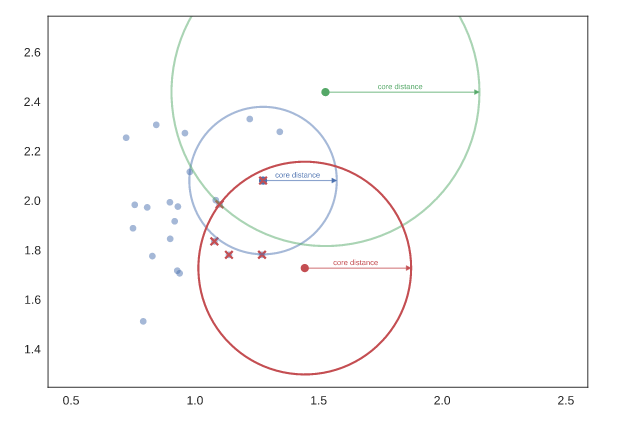
\includegraphics[width=0.5\textwidth]{hdbscan_1}
    \caption{The core distances. TODO give more detailed explanation.}
    \label{fig:hdbscan_1}
\end{figure}

Once the core distances are known, the mutual reachability distance between two points is defined as follows:

\begin{equation*}
    d_{mreach}(a, b) = max\{core_k(a), core_k(b), d(a, b)\}
\end{equation*}

where $d(a, b)$ is the original distance between $a$ and $b$. Therefore if two points are close together, but the density around one point is rather low, the core distance will be greater than the original distance and thus the two points appear to be less close together when considering the mutual reachability distance.

\subparagraph{2. Build the minimum spanning tree}

Based on the mutual reachability distances, the next step is to find points close  to each other. This is done by creating a minimum spanning tree, where edges are weighted according to the mutual reachability distance and a point is represented by a vertex. The minimum spanning tree is created one edge at a time, always choosing the lowest distance to a vertex not yet in the tree. This is done until each vertex is connected, which results in the minimal set of edges, such that dropping any edge will cause the disconnect of one or more vertices from the tree.

\subparagraph{3. Build the cluster hierarchy}

Once the minimum spanning tree is complete, it is converted into a hierarchy of connected clusters, by sorting edges of the tree by distance and iterate through, creating a new merged cluster for each edge. The dendogram in Figure \ref{fig:hdbscan_2} shows a possible cluster hierarchy. %TODO rewrite this paragraph. 

\begin{figure}[h]
    \centering
    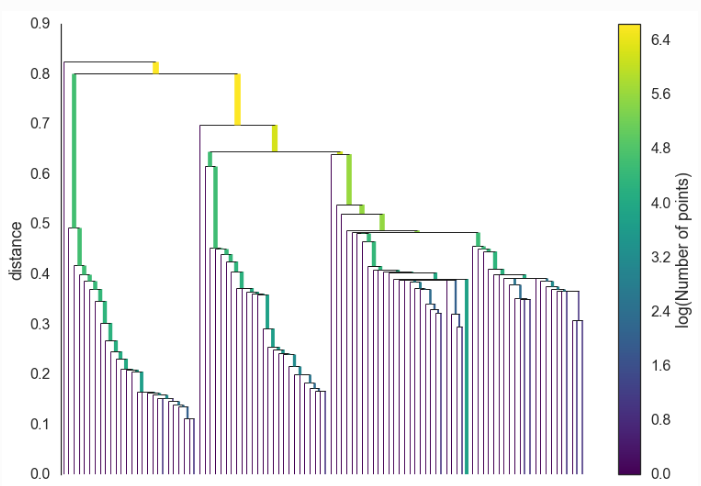
\includegraphics[width=0.5\textwidth]{hdbscan_2}
    \caption{The cluster hierarchy shown as a dendogram}
    \label{fig:hdbscan_2}
\end{figure}

At this stage we have to flatten the hierarchy to get the final clusters, which provide the best representation of the current data set. DBSCAN simply cuts through the hierarchy using a fixed parameter, usually called epsilon, to get the final clusters. This approach does not work well with clusters of varying densities and the epsilon parameter itself is unintuitive, requiring further exploration to find optimal values. This is were HDBSCAN improves upon DBSCAN, by taking additional steps for finding relevant clusters.

\subparagraph{4. Condense the cluster tree}

\begin{figure}[h]
    \centering
    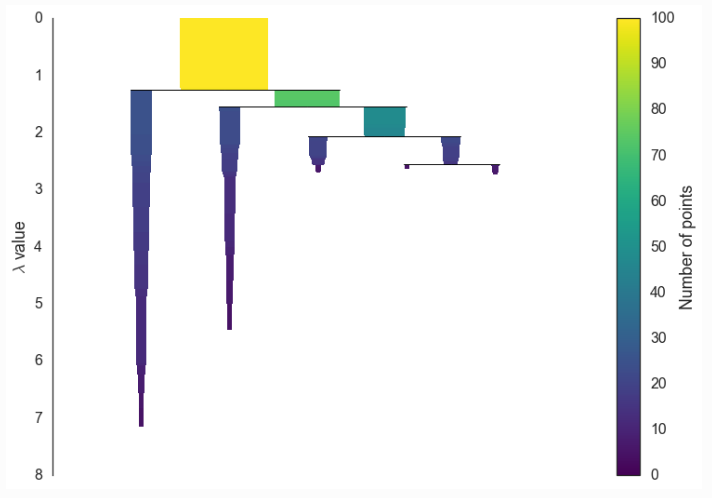
\includegraphics[width=0.5\textwidth]{hdbscan_3}
    \caption{Condensed cluster hierarchy}
    \label{fig:hdbscan_3}
\end{figure}

The fourth step consists of condensing the previously built cluster hierarchy into a smaller tree. The process starts at the top where all vertices still belong to the same cluster. Iterating through the hierarchy, for each split the two resulting clusters are compared against a predefined minimum cluster size. If the size of a cluster is below the minimum, its points will be discarded, while the other cluster remains in the parent cluster. If both cluster sizes are above or equal the minimum, the clusters are considered as true clusters. This is repeated until no more splits can be made. 


\subparagraph{5. Extract the clusters}

The extraction of the final clusters from the condensed tree is based on the stability per cluster and once it is selected, none of its subclusters can be chosen. The stability is based on the persistence of a cluster, which is measured by $\lambda = \frac{1}{distance}$. The stability for a cluster $C$ is defined as

\begin{equation}
\sum_{p \in \text{C}}^{|C|} ({\lambda}_{p} - {\lambda}_{birth})
\end{equation}

 where ${\lambda}_{p}$ describes when point $p$ fell out of the cluster and $ {\lambda}_{birth}$ describes when the cluster was created. Now calculating the stability for each cluster starts at the leaf nodes and ends when the root is reached. A cluster is selected if its stability is larger the sum of stabilities of its children. If the sum child stabilities is larger than that of its parent, the parent stability will be set to the value of the sum of its children, but no selection will be done. Based on this approach the final clusters will be selected, with regards to varying densities and noise.